% !TEX root = ../main.tex
\section{基于禁忌搜索的CNC工序分配}
	\subsection{模型的假设与标记}
		\subsubsection{假设}
			\begin{enumerate}
				\item\label{刀具}假设CNC在一班次连续作业中不能更换刀具,即一班次连续作业中一台CNC只能执行一道工序。
			\end{enumerate}
		\subsubsection{标记}
			\begin{table}[htbp]
				\centering
				\caption{标记:针对非抢占式排队系统的静态调度模型}
				\label{标记:针对非抢占式排队系统的静态调度模型}
					\begin{longtabu}to\linewidth{@{}X[c]|X[l]@{}}
						\toprule
						变量&定义\\\midrule
						\(m\)&工序总数\\
						\(n\)&CNC总数\\
						\(T_{\mathrm{RGV}_i}\)&RGV在第\(i\)道工序时的机器周期\\\bottomrule
					\end{longtabu}
			\end{table}
	\subsection{模型的建立与求解}
		\subsubsection{建立}
			如公式\ref{不同工序的机器周期公式},当CNC的加工分为不止一个工序时,RGV在每道工序的机器周期是不一样的。只有在最后一道工序时才需要清理。
			\begin{align}
				\label{不同工序的机器周期公式}
				T_{\mathrm{RGV}_i}&=T_\mathrm{ready}+T_\mathrm{move}+T_\mathrm{update}&i=1..m-1\\
				T_{\mathrm{RGV}_m}&=T_\mathrm{ready}+T_\mathrm{move}+T_\mathrm{update}+T_\mathrm{clean}&
			\end{align}
			\par\indent 根据假设\ref{刀具},CNC可加工的工序在一开始就已经被确定。对于\(m\)道工序和\(n\)台CNC的情况,一共有\(m^n\)种可能。考虑到解的取值个数随输入呈指数级增长,复杂情况下求最优解运算量过大且不易实现,有必要使用启发式算法\cite{陈华孙启元-392}。选用全局逐步寻优的禁忌搜索,既减小了运算量,也在一定程度上保证了解的质量。
			\begin{figure}[htbp]
				\centering
				\caption{程序流程图:基于禁忌搜索的CNC工序分配}
				\label{程序流程图:基于禁忌搜索的CNC工序分配}
				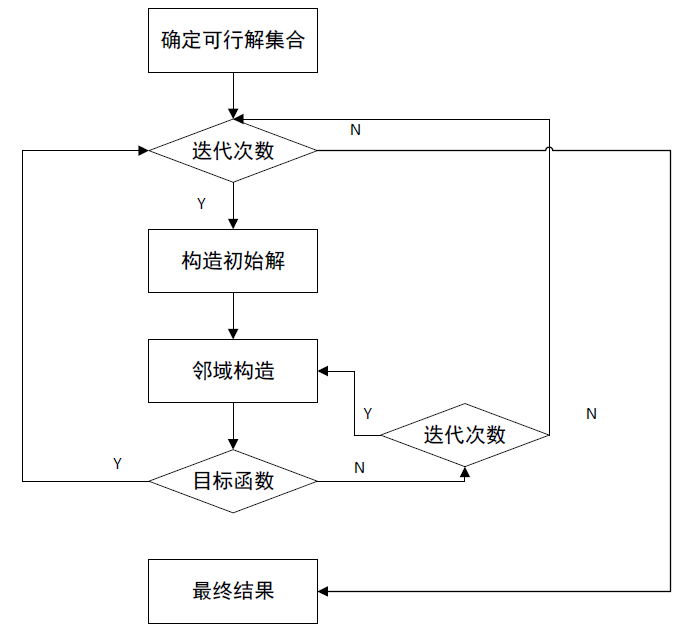
\includegraphics[width=10cm]{graph/flow.png}
			\end{figure}
			\paragraph{禁忌搜索}如图\ref{程序流程图:基于禁忌搜索的CNC工序分配}。
			\begin{enumerate}
				\item 确定可行解集合、当前最优解以及目标函数;
				\item 判断迭代次数,若尚未达到则继续执行,否则输出当前最优解;
				\item 以当前最优解为基础,通过邻域构造法(即任意改某一台CNC加工工序属性或交换任意两台CNC位置)创造候选解,若候选解属于可行解则构造成功,反之重新构造;
				\item 计算候选解目标函数值,并与当前最优解进行比较,若优于当前最优解则替代,否则进入步骤五;
				\item 判断邻域构造迭代次数,若尚未达到则执行步骤三继续构造候选解,否则执行步骤二。
			\end{enumerate}
			\par\indent 考虑到禁忌搜索的效率很大程度上取决于可行解集合的大小以及当前最优解的质量,因此针对确定的RGV初始位置以及加工工序时间,确立两个可能解的条件:
			\begin{enumerate}
				\item CNC平台占比与加工工序时间成正比,即加工时间长的工序,其所配置的CNC平台数量应相对较多;
				\item 执行第一道工序的CNC平台应靠近RGV初始位置;
			\end{enumerate}
			\par\indent 根据这两个可行解的条件能够大大减小可行解数量。
			而当前最优解可以确定为
			\begin{enumerate}
				\item 不同工序分配比例即为不同工序时间的比例;
				\item 执行第一道工序CNC位置靠近RGV初始位置,且不同工序由近到远循环排列。
			\end{enumerate}
			\par\indent 例如8台CNC两道工序对应当前初始解为12121212式排列。
		\subsubsection{求解}
			程序清单\ref{主程序}和程序清单\ref{穷举搜索最优CNC工序分配分布}给出了利用穷举算法求出的最优分配分布。求解结果见运行结果\ref{穷举搜索最优CNC工序分配分布结果}。而程序清单\ref{模拟退火搜索最优静态调度和最优CNC工序分配分布的主程序}和\ref{模拟退火搜索最优静态调度和最优CNC工序分配分布}通过启发式算法给出了一个计算时间较短的解。
